\section{Vissim Network Modelling}
\label{modelling}
The Vissim network used throughout the project is derived from a network originally started COWI and later reworked by DTU Transport students.

COWI's version included O3 from Jyllingevej to the intersection with highway 3 and even further north. In addition highway 3, which runs almost parallel with O3 in this area, was included as well as the minor roads in between.
The network was setup with dynamic assignment of traffic.

\subsection{Modifications \& Additions to Existing Model}

As such the network was missing four intersections of O3 from Jyllingevej to Roskildevej. To establish this section satellite photos from Google Earth was combined with intersection layouts, kindly provided by DRD.

The signal plans and naming conventions for the existing intersections in the COWI model for O3 intersections were adopted when entering the four missing intersections into the network. As for the intersection layout, DRD provided the missing signal plans for these intersections as well.

To prevent side-effects all links not connected to O3 from Herlev Sygehus to Jylligevej were removed as well as all parking lots (DTA zones).

\subsection{Link Inputs}

Due to the arterial nature of the Herlev area there is a natural distinction between major and minut link inputs. The major inputs are positioned in the ends and minor inputs are placed for each minor road.

In the southgoing direction vehicles entering the arterial from highway 3 and the northern extension of O3 are represented by a single input positioned before the intersection at Herlev Sygehus and would be detected by D3.

Northgoing traffic input is defined on the link leading to the Mileparken intersection and is detected by D14. 

The relative size of the major inputs are set according to the relative directional distribution seen in Figure \ref{fig:herlev_props} ie. 45\% northgoing and 55\% southgoing. XXX Insert more specific figure XXX

As the available dataset does not include detectors on the minor sideroads - from either side of the arterial - it is difficult to assess the relative size of the inputs from them. Thus for the remaining roads adjacent to the arterial are defined minor input links of identical size with the exception of the Herlev Sygehus link, which is set to be double the size to match the observations made above.
It is arguable that much traffic enters at the Herlev Hovedgade intersection, but the detected traffic does not indicate that this is significant.

The combined traffic input is set so that in total 20\% arise from the minor roads and the remainder enters from the ends of the arterial. 

XXX Try to find something to back this up eg. from Steen Lauritzens report XXX.

\subsection{Routes}
At every intersection it is possible to follow each adjacent link (ie. turn left, right or go straight through). The lack of a full detector dataset from the area prevents determination of the exact distribution of input on the possible routes. In addition, since it is possible to reach almost every output link from an input link, some simplifying conditions were selected to solve the problem with lack of data and the large number of routes.

It was decided that input from minor roads should turn onto the arterial and choose a north- or southgoing route to the respective end of the arterial with equal probability ie. turn-in traffic does not turn out again but continue along the arterial. In Vissim this effect is accomplished by simply omitting route assignment for vehicles entering on minor links.

To represent turn-out traffic routes choices are inserted for the major inputs only. Thus, from either end of the arterial, there is a route, which turns out, at each intersection in addition to a route going straight-through. 

The proportions for turn-out routes are choosen identical to those of the relative input size for the minor links, which are chosen after the arterial. This coincides with the total traffic input so that 80\% of the traffic goes straight through and 20\% turns out.

\subsection{Signal Plans}
Signal plans define the stage sequence, green duration and how changes between adjacent stages should happen with respect to colors in the from and to stages. For cycle-based signal plans the cycle time must be equal to the sum of green and interstage time from the beginning of the first stage until it begins again.

A single stage defines the signal head colors of one or more signal group, which, in turn, is a group of signal heads operating synchronously.

The simplest signal controller consist of two stages. In  Figure \ref{fig:simple_intersection} the arrows indicate the directions being served green.

\begin{figure}[!ht]
\begin{center}
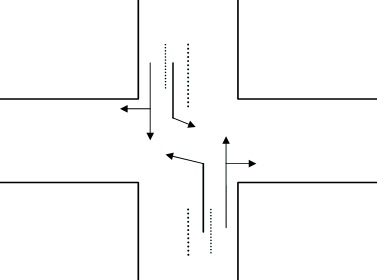
\includegraphics[scale=0.5]{simple_intersection.png} 
\end{center}
\caption{A simple intersection}
\label{fig:simple_intersection}
\end{figure}

DOGS rely on existing signal and modify the duration of the stage or stages, which serve green in the direction of the arterial. Thus DOGS assume that the stage sequence and interstages are \textit{optimized} so that the time lost in stage changes is minimized and \textit{safe} so that vehicles in eg. left-turning movements have time to leave the intersection before the conflicting direction receives green.

For this project DRD has supplied a number of signal plans for each intersection, developed by TTS. Throughout the plans signal groups in one direction (usually the major one) are named A and B in the perpendicular direction. Names such as At, AV, AtV indicates signal group for the throughgoing, leftgoing (V = venstre (danish) = left) and a combination for the final name variant. Lower case a's and b's indicate a signal group for pedestrians in the major and minor direction resp.

For some intersections a number of alternative plans were supplied. Considering the scope of this project only a single plan was chosen for each intersection and time of day. Generally plans involving pedestrian or bicyclist actuated stages were avoided so as to maximize the potential for traffic signal optimization. It was confirmed by TTS that these types of stages, which are taken in a stochastic manner ie. when a button is pressed, can be devastating to the coordination of traffic signals.

As a final simplifying step it was chosen not to provide signal heads for pedestrians and bicyclists as these types of road users are not being simulated. Pedestrian stages will mostly follow the parallel stages anyway and if this is not the case the stage, which is being denied in favor of the pedestrian stage, will simply receive red for the duration.

The final plans, which are used in the simulation, can be seen in appendix \ref{app:signalplans}.

The actual implementation was done in VAP by running the interstages at the cycle second according to the signal plan, for more details refer to section \ref{vap}.

\subsection{Route Fractions from Traffic Counts}
\label{routefractions}
The Vissim manual is very clear that static routes should be used over turning decisions, mainly because congestion may cause a decision to turn to be overruled whereas a vehicle on a fixed route will wait for the congestion to clear.

In the beginning of each input link a routing decision is placed so that every vehicle in the network is following a route. The question remains how many should follow each route.

DRD supplied traffic counts for all intersections with the exception of Ejby Torvevej, which is blinded from east and is estimated by DRD to contribute very little.

The counting period was 7.00-9.00 in the mornings and 15.00-17.00 in the afternoons in 15-minutes intervals. The counts involved, for each approach, the turning movements of cars (including vans) and trucks. 

Traffic counts only show how flow traverses the individual intersection. In order to gain relative route distributions from these traffic counts a linear programming (LP) model by Jesper Larsen was implemented. The solutions to the model will give the relative fraction 

Routes are modelled as strings of turning decisions. Each time an intersection is reached a it must be decided which direction to take next, for example left, right of through (whichever is applicable). Such decision happen at a \textit{decision point}.

The model consist of a few constraints which much be satisfied by assigning values to $\mathbf{r}$, the relative route loads.

\begin{table}[!ht]
\begin{center}
\begin{tabular}{ll}
\hline
$k = 1...m$ & Route indexes \\
$l = 1...n$ & Decision point indexes  \\
$j = 1...c_l$ & Indexes of direction alternatives at the $l$'th decision point  \\
$D$ & Decision points. Columns represent routes and rows the decisions  \\
$P$ & Relative input distribution between adjacent decision points  \\
\hline
\end{tabular}
\end{center}
\caption{Notation for turning probabilities to route fraction model}
\end{table}

\begin{eqnarray}
D_{l,j} \cdot r_k = y_l \cdot p_j & \forall l,j,k \\
y_l = \sum_{i = 1}^{n}{P_{i,l} \cdot y_i} & \forall l
\end{eqnarray}

Where $m$ is the number of routes and $n$ is the longest string of choices. The matrix P indicates how the input to the decision point at row $i$ is distributed to decision points $l$. Thus P contains the turning probabilities from our traffic counts and may look like Figure \ref{fig:flow_dist_principle}. Below is the matrix form of this model.

\begin{eqnarray}
\mathbf{D} \cdot \mathbf{r} = \mathbf{y} \cdot \mathbf{p} \\
\mathbf{y} = \mathbf{P} \cdot \mathbf{y}
\end{eqnarray}

\begin{figure}[!ht]
\begin{center}
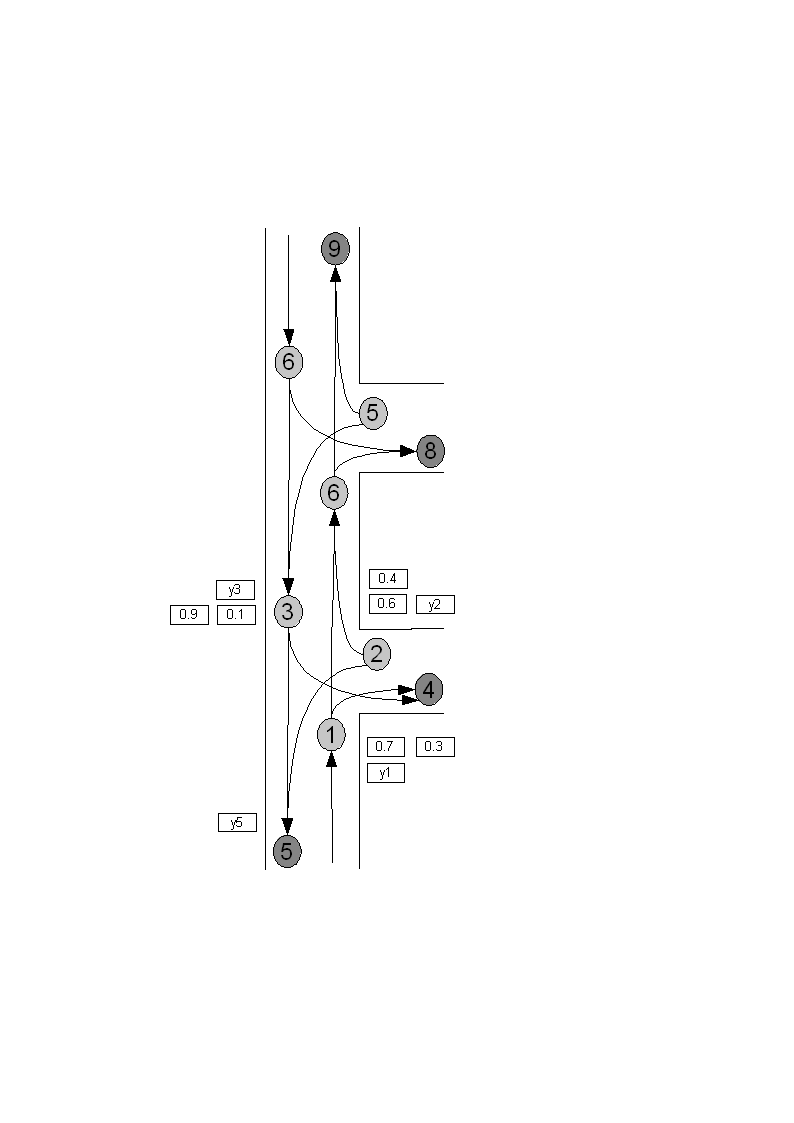
\includegraphics[scale=0.6]{trafficcount_to_routes_sketch.png} 
\end{center}
\caption{Flow distribution principle}
\label{fig:flow_dist_principle}
\end{figure}

In Table \ref{tbl:flow_dist_principle} is a selection of the $P$-matrix which corresponds to this network layout and turning probabilities.

The downstream input is calculated by summing the upstream inputs multiplied by the turning percentages for the directions facing the decision point. For example $y_5 = 0.6 y_2 + 0.9 y_3$. In this case $y_2$ is an input link (same as 1, 5 and 6) with direct input defined per-hour i Vissim and $y_3$ is derived from the upstream inputs and turning probabilities name input and left-turning probability on link 5 and input and through-going probability on link 6.

\begin{table}[!ht]
\begin{center}
\begin{tabular}{l|ccc}
 	& 4 & 5 & 6 \\ \hline
1	& $0.3$ & 0 & $0.7$ \\
2	& $0.6$ & 0 & $0.4$ \\
3	& $0.1$ & $0.9$ & 0
\end{tabular}
\end{center}
\caption{Example of input distribution using turning percentages. Rows are donors and columns are recipients. The row-sums must be $1.0$ to illustrate that all input is distributed and is not \textit{lost} in the intersection and no decision point must distribute input to itself.}
\label{tbl:flow_dist_principle}
\end{table}

